%% 
%% This is a sample doctoral dissertation.  It shows the appropriate
%% structure for your dissertation.  It should handle most of the
%% strange requirements imposed by the Grad school; like the different
%% handling of titles of one/many appendices.  It will automatically
%% handle the linespacing changes.  The body default is double-spaced
%% (except when you use the singlespace or condensed options).  The
%% default for quotations is single-space, and the default for tabular
%% environments is also single-space.  
%%
%% This class adds the following commands and environments to the
%% report class, upon which it is based:
%% Commands
%% ------------
%% \degree{name}{abbrv} -- Sets the name and abbreviation for the degree.
%%                         These default to ``Doctor of Philosopy''
%%                         and ``Ph.D.'', respectively.
%% \copyrightyear{year} -- for the copyright page.
%% \bachelors{degree}{institution} -- for the abstract
%% \masters{degree}{institution}   --  "
%%     if you have other degrees you may use
%% \secondbachelors{degree}{institution}
%% \thirdbachelors{degree}{institution}
%% \secondmasters{degree}{institution}
%% \thirdmasters{degree}{institution}
%% \priordoctorate{degree}{institution}
%%
%% \committeechair{name}           -- for the signature page
%% or, if you have two co-chairs:
%% \cochairs{first name}{second name}
%%
%% \firstreader{name}              --  "
%% \secondreader{name}             --  "
%% \thirdreader{name}              -- (optional)
%% \fourthreader{name}             --  "
%% \fifthreader{name}              --  "
%% \sixthreader{name}              --  "
%% \departmentchair{name}          -- for the signature page
%% \departmentname{name}           --  "
%%
%% \copyrightpage                  -- produces the copyright page
%% \signaturepage                  -- produces the signature page
%%
%% \frontmatter                    -- these are required in their various
%% \mainmatter                     -- appropriate locations
%% \backmatter                     --
%%
%% \unnumberedchapter[toc]{name}   -- like \chapter, except that it
%%                                    produces an unnumbered chapter;
%%                                    alternatively, like \chapter*,
%%                                    except that it lists the chapter
%%                                    in the table of contents.
%%
%% New environments:
%%   dedication  -- for the dedication
%%   abstract    -- for the abstract
%%
%% The thesis documentclass is built on top of the report document class.
%% It accepts all of the options that the report class accepts, plus the
%% following:
%%     doublespace -- the default, indicates double spacing as per U.Mass.
%%                    requirements.  You will need this when you do your
%%                    final copy.
%%     singlespace -- for earlier work, not acceptable to the Grad school
%%     condensed   -- for earlier work, not acceptable to the Grad school,
%%                    creates condensed versions of the frontmatter. 
%%                    Condensed implies singlespace.
%%     dissertation - the default, indicates that this document is a
%%                    dissertation.
%%     proposal    -- indicates that this document is a dissertation proposal,
%%                    rather than a dissertation.  This will only change the
%%                    wording on the title and signature pages.
%%     thesis      -- indicates that this document is a Master's thesis 
%%                    rather than a doctoral dissertation.  This also changes
%%                    the default for \degree to Master of Science, M.S.
%%     allowlisthypenation -- (the default), allows hyphenation of words in
%%                    the table of contents, the list of figures, and the list
%%                    of tables.  I believe that this is acceptable to the 
%%                    Graduate School.
%%     nolisthyphenation -- disallows hyphenation of words in the table of
%%                    contents and the list of figures and tables.  Use this 
%%                    option if the Grad School doesn't like your hyphenation.
%%     nicerdraft  -- relaxes some of the Grad School's rules for working with
%%                    drafts -- has no effect when doublespace is in effect
%%     nonicerdraft -- the default, leaves things in draft as they will be in
%%                     the final version
%% umthesis changes the default font size to 12pt, but you may specify 10pt or
%%   11pt in the options.
\documentclass[dissertation]{umthesis}          % for Ph.D. dissertation or proposal
% \documentclass[thesis]{umthesis}  % for Master's thesis
\usepackage{graphicx}
\usepackage{caption}
\usepackage{subcaption}
\usepackage{color}

%%
%% If you have enough figures or tables that you run out of space for their
%% numbers in the List of Tables or List of figures, you can use the following
%% command to adjust the space left for numbers.  The default is shown:
%%
%% \setlength{\tablenumberwidth}{2.3em}

%% Use the hyperref package if you're producing a version for online
%% distribution and you want hyperlinks.  Note that the Grad School doesn't want
%% their PDF viewers to colorize or otherwise highlight the links; use the
%% hidelinks option to hyperref to avoid decorating links.
%\usepackage[hidelinks]{hyperref}


%%%%%% added by Laura 10/22-24
\usepackage{hyperref}  % makes references clickable in the pdf, very useful!
\usepackage{rotating}
\usepackage{ulem} \normalem 
\newcommand{\laura}[1]{{\color{blue}{#1}}}
\newcommand{\LC}[1]{{\color{magenta}{[[LC #1]]}}}
\providecommand{\todo}[1]{{\color{red}$\blacksquare$~\textsf{[TODO: #1]}}}

\def\imbh#1{intermediate mass black hole#1(IMBH#1)\gdef\imbh{IMBH}}
\def\smbh#1{supermassive black hole#1(SMBH#1)\gdef\smbh{SMBH}}
\def\bbh#1{binary black hole#1 (BBH#1)\gdef\bbh{BBH}}
\def\bh#1{black hole#1 (BH#1)\gdef\bh{BH}}
\def\ns#1{neutron star#1 (NS#1)\gdef\ns{NS}}
\def\gw#1{gravitational wave#1 (GW#1)\gdef\gw{GW}}
\def\sn#1{core-collapse supernova#1 (CCSN#1)\gdef\sn{CCSN}}
\def\pnw#1{post-Newtonian#1 (PN#1)\gdef\pnw{PN}}
\def\eos#1{equation of state#1 (EOS#1)\gdef\eos{EOS}}
\def\grb#1{gamma-ray burst#1 (GRB#1)\gdef\grb{GRB}}
\def\amr#1{adaptive mesh refinement#1 (AMR#1)\gdef\amr{AMR}}
\def\isco#1{innermost stable circular orbit#1 (ISCO#1)\gdef\isco{ISCO}}
%%%%%%%%%%%%%%%%%%%%%%%

\begin{document}

%%
%% You must fill in all of these appropriately
\title{The impact of terrestrial noise on the detectability and reconstruction of gravitational wave signals from core-collapse supernovae}
\author{Jessica L McIver}
\date{March xx, 2015} % The date you'll actually graduate -- must be
                     % February, May, or September
\copyrightyear{2013}
\bachelors{B.S. Physics}{Syracuse University}
\secondbachelors{B.S. Magazine Journalism}{Syracuse University}
\masters{M.S. Physics}{University of Massachusetts Amherst}
\committeechair{Laura Cadonati}
\firstreader{Alexandra Pope}
\secondreader{David Kastor}
\thirdreader{Benjamin Brau}
\departmentchair[Department Head]{Rory Miskimen} % Uses "Department Chair" as the title. To
% use an alternate title, such as "Chair", use \departmentchair[Chair]{Pete Shearer}
\departmentname{Physics}
\degree{Doctor of Philosophy}{Ph.D.}

%%
%% These lines produce the title, copyright, and signature pages.
%% They are Mandatory; except that you could leave out the copyright page
%% if you were preparing an M.S. thesis instead of a PhD dissertation.
\frontmatter
\maketitle
\copyrightpage     %% not required for an M.S. thesis
\signaturepage

%%
%% Dedication is optional -- but this is how you create it
%\begin{dedication}              % Dedication page
%  \begin{center}
%    \emph{To those little lost sheep.}
%  \end{center}
%\end{dedication}

%%
%% Epigraph goes here...(aka frontispiece)
%% \chapter{Epigraph}?????

%%
%% Acknowledgements are optional

% \chapter{Acknowledgements}             % Acknowledgements page
%Thanks to XX for very extensive comments that have greatly improved this proposal. \
%Prof. Laura Cadonati  
%Dr. James Clark
%Sarah Gossan 
%Duncan Macleod 
%Josh Smith 
%Jeff Kissel 
%Brian Lantz
%Claudia Lazzaro 
%Florent Robinet 
%Thank committee 
% 
%Laura Nuttall 
%Marissa Walker
%Thomas Abbott
%TJ Massinger 
%Chris Pankow 
%Peter Saulson 
%Gaby Gonzalez 
%Hugh Radkins 
%Rich Mittleman 
%Sarah Zuraw
%Kalina Nedkova 


%%
%% Abstract is MANDATORY. -- Except for MS theses
\begin{abstract}                % Abstract

Gravitational waves, tiny ripples in the fabric of spacetime, will offer insight into some of the most interesting and energetic astrophysical phenomena, like black hole coalescence and core-collapse supernovae. The Advanced Laser Interferometer Gravitational wave Observatories (aLIGO) are poised at the brink of discovery, about to begin the first observing runs with newly upgraded instrumentation. 

The recently installed new hardware promises a ten-fold improvement in LIGO's astrophysical observation range, but also the challenge of understanding unexpected sources of noise and how they will affect searches for gravitational wave transients.
In this work I will focus on one potential \gw{} source of great interest for aLIGO: core-collapse supernovae, 
violent star deaths that are some of the most energetic events in the Universe. The inner mechanics of these supernovae are obscure to optical telescopes, and the only way to gain insight into the explosion mechanism driving these events is to infer the intricate interior dynamics of these supernovae through direct observation of gravitational waves, or learn about the pre-collapse thermodynamics with low-energy neutrino observation. 
\\
I will present an overview of current \sn{} models, the state of model selection research, and the broader applications of improving waveform reconstruction techniques for longer duration signals with rich and complex structure. I present results for the performance of current waveform reconstruction pipelines using \sn{} waveforms based on these models, and show the adverse affect that the introduction of non-Gaussian noise artifacts presents.\\
% 
For any transient \gw{} signal, a crucial component to both earliest possible detection and our understanding of candidate events is the characterization of early data from Advanced LIGO detectors. I present also an overview of the impact of terrestrial noise on the detectability and reconstruction of astrophysical \gw{} transients. Much focus is devoted to elevated levels of transient ground motion - a particularly egregious problem in past science runs. A brief overview of seismic isolation configuration used for the Advanced LIGO instruments is presented. Results show the mitigation of transient noise is effective in reducing transient noise amplitude in the GW band, but not in reducing transient rate during periods of elevated ground motion. 
%- 

%




\end{abstract}

%%
%% Preface goes here...would be just like Acknowledgements -- optional
%% \chapter{Preface} 
%% ...


%%
%% Table of contents is mandatory, lists of tables and figures are 
%% mandatory if you have any tables or figures; must be in this order.
\tableofcontents                % Table of contents
%\listoftables                   % List of Tables
\listoffigures                  % List of Figures

%%
%% We don't handle List of Abbreviations
%% We don't handle Glossary

%%%%%%%%%%%%%%%%%%%%%%%%%%%%%%%%%%%%%%%%%%%%%%%%%%%%%%%%%%%%%%%%%%%%%%%%%
%% Time for the body of the dissertation
\mainmatter   %% <-- This line is mandatory

%%
%% If you want an introduction, which is not a numbered chapter, insert
%% the following two lines.  This is OPTIONAL:
%\unnumberedchapter{Introduction}
%Why on earth do I want to study sheep anyway?

%%
%% Some sample text
\newpage
\chapter{Introduction }

\section{Overview}
\subsection{Gravitational waves - a new window to the Universe}

Astrophysics overview - what could we see?  
\subsection{Core collapse supernovae} 
%
%%
\subsection{LIGO and Advanced LIGO} 
The LIGO interferometers are built to sense gravitational waves by measuring strain, or the change in length over the length of two 4km perpendicular arms. To accomplish this, a 1064~nm laser beam is split down each of the arms, reflected back via high reflectivity mirrors, and recombined. Any change in relative length between the arms will change the interference pattern for the recombined light, and we can infer the dynamics of the astrophysical source from the space-time perturbation manifested in this strain.

Searches for generic \gw{} transients, or \textit{bursts}, in data from previous LIGO science runs were able to make new and astrophysically meaningful upper limit statements (\cite{Vela}, \cite{BurstAllSky}, \cite{GRBs}), but their reach was limited by fundamental sources of noise, such as seismic, thermal, and shot noise as seen in Figure \ref{fig:iLIGO}.

\begin{figure} 
\centering
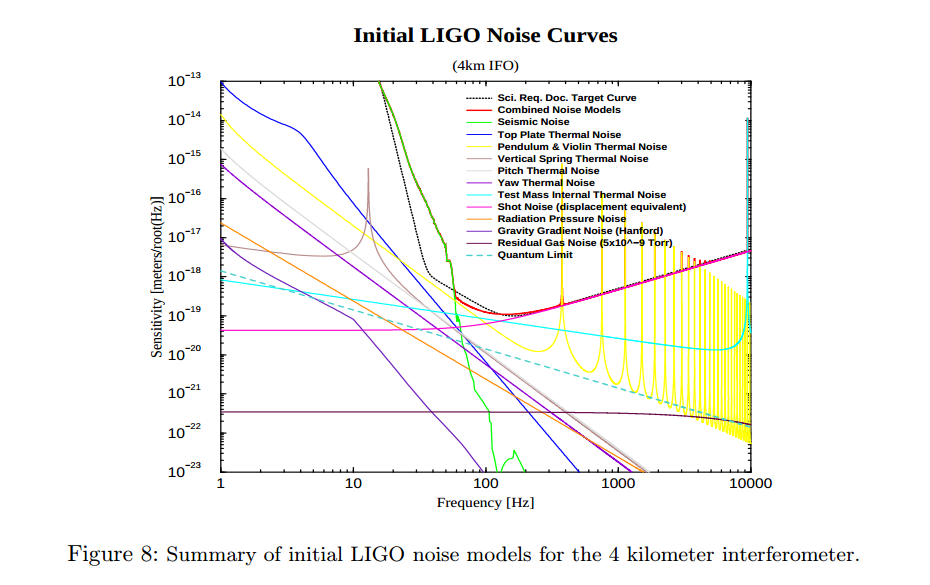
\includegraphics[width=\linewidth]{figures/iLIGO_noise_curve.png}
\caption{Fundamental sources of noise for iLIGO. Note the science requirement curve denoted with a dotted black line, the iLIGO combined noise curve in red, seismic noise in green limiting at lower frequencies, thermal noise in yellow limiting about 100Hz, and shot noise in magenta limiting at higher frequencies \cite{iLIGO_poster}.} 
\label{fig:iLIGO_noise}
\caption{Fundamental noise sources and their contribution to sensitivity in various frequency regimes.}
\label{fig:iLIGO} 
\end{figure}

\subsection{Extracting CCSN physics from Advanced LIGO data} 
\subsubsection{Detectability} 
\subsubsection{Waveform reconstruction}
extraction of rich, complex information

\subsection{Terrestrial sources of aLIGO noise and their impact on CCSN}
\subsection{Common sources of noise} 
\subsection{Transient noise}
\subsection{Seismic noise}
Seisveto paper - S6 DetChar 
\subsection{Terrestrial noise: impact on detectability, parameter estimation, and waveform reconstruction }
S6 all sky DQ 
NINJA2 results - glitches obscure parameter estimatio


%
%%
\section{General Relativity and Gravitational waves} 
\subsection{Prediction of gravitational waves} 
\subsection{Propagation of gravitational waves}
\subsection{Gravitational wave astronomy}

%
%%
\section{LIGO and Advanced LIGO}

 
\subsection{Advanced LIGO}

To combat noise sources that limited \gw{}  searches in previous science runs, the LIGO detectors are currently undergoing an instrumentation upgrade to Advanced LIGO, including the installation of active seismic isolation and improved suspensions systems for each mirror as well as improvements to the optics and laser subsystems \cite{Harry-aLIGO}. Advanced LIGO data will be usable for \gw{}  searches down to 10 Hz; a 30 Hz improvement over initial LIGO (compare Figures \ref{fig:iLIGO_noise} and \ref{fig:aLIGO_noise}). 

\begin{figure} 
\centering
\begin{subfigure}{.48\textwidth}
  \centering
  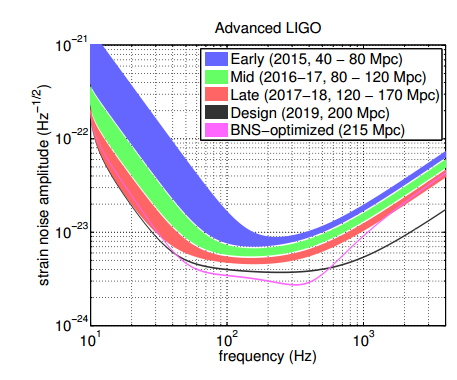
\includegraphics[width=\linewidth]{figures/aLIGO_noise_curve.png}
  \caption{The expected noise curves for different stages of Advanced LIGO science run data taking \cite{aLIGOoutlook}}. 
  \label{fig:aLIGO_noise}
\end{subfigure}%
\quad
\begin{subfigure}{.48\textwidth}
  \centering
  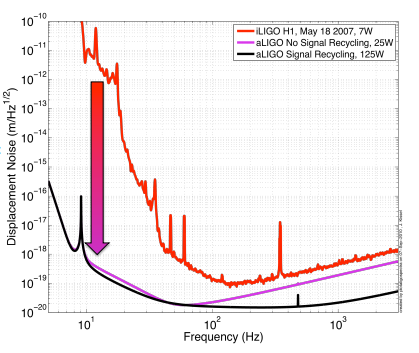
\includegraphics[width=\linewidth]{figures/aLIGO_performance_gain.png}
  \caption{The performance gained at 10Hz with new aLIGO seismic isolation instrumentation. \cite{KisselThesis}. Credit: J. Kissel.} 
  \label{fig:SEISUSgain}
\end{subfigure}
\caption{A comparison of anticipated Advanced LIGO noise curves, highlighting the improvement at low frequencies.}
\label{fig:aLIGO} 
\end{figure}

The Advanced LIGO detectors are quickly completing construction, installation, and testing and there could be a second generation interferometric \gw{} science run as soon as 2015 with Advanced Virgo following shortly after in 2016 (see Appendix for discussion of global interferometer network). The next two years are a key time to be exploring interesting potential \gw{}  sources and tuning our new instrumentation to optimize the potential for scientific discoveries. 

Characterization of the instrument before these science runs begin is crucial to making the first \gw{}  detection. The new Advanced LIGO instrumentation reduces seismic noise by six orders of magnitude at 10Hz and thermal noise by a factor of 10 around 100Hz (see Figure \ref{fig:SEISUSgain}). This brings Advanced LIGO closer to being a quantum limited detector, but introduces many new potential glitch mechanisms. 


\subsection{The LIGO interferometers and the global interferometer network}

There are two 4km LIGO interferometers - one in Livingston, Louisiana and one in Hanford, Washington. The hardware belonging to a third LIGO interferometer is in the process of being transferred to India. The 3km Virgo detector in Italy is also undergoing similar hardware upgrades to Advanced Virgo, the underground cryogenic detector KAGRA is being built in Japan, and the 600m GEO600 detector in Germany is testing new technology planned for future upgrades like light squeezing. Together, this network of advanced interferometers will increase sensitivity to gravitational waves tenfold and enable significantly improved sky localization \cite{Gonzalez-GWA}. 

\subsection{Advanced LIGO seismic isolation} 

Advanced LIGO features new complex instrumentation that needs to be carefully characterized: a 10-times more powerful laser, a new thermal compensation system, new suspensions, and an active seismic isolation. To prepare all subsystems, the detector characterization working group has appointed subsystem leads to direct characterization efforts for these subsystems and liaison with the commissioners and engineers. I have been serving as the seismic isolation subsystem lead for about a year and a half now, leading a team of a dozen researchers in projects aimed to better understand the seismic isolation performance and how it affects the \gw{} searches. 

It may seem nonintuitive that excess seismic noise, which limits the search range only at frequencies below 10 Hz, according to Figure \ref{fig:aLIGO_noise}, would be a candidate for interfering with transient \gw{}  searches above 40 Hz. However, local ground motion was one of the limiting noise sources in searches for transient \gw{}  sources during previous LIGO science runs (2005--2010). Seismic noise has been shown to couple with transient searches via an up-conversion mechanism (or mechanisms) that hasn't been well identified~\cite{Macleod-Seisveto}. 

For average motion, the Advanced LIGO active seismic isolation systems are designed to push the lower frequency bound of aLIGO sensitivity to the technological limit (see Figure \ref{fig:SEISUSgain} for a depiction of the improvements aLIGO is expected to achieve with this new instrumentation). 
The active seismic isolation systems are composed of several mechanically isolated platforms, known as stages - as seen in Figure \ref{fig:BSC_ISI}. To reduce seismic noise, the motion of each stage is measured with respect to the stage below it and controlled with precise, powerful actuators with a well-tuned feedback loop to remain as stationary as possible - as in Figure \ref{fig:SEI_iso} \cite{KisselThesis}. 

\begin{figure}[htb]
	\center{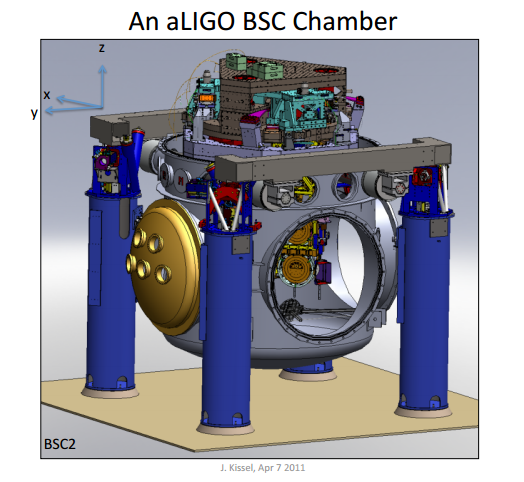
\includegraphics[scale=0.55]
	{figures/BSC_ISI.png}}
	\caption{\label{fig:BSC_ISI} A representation of the Advanced LIGO active isolation platforms and suspensions for the core optics. The Hydraulic External Pre-Isolator (HEPI) is in dark blue, the Internal Seismic Isolation (ISI) stages are in grey and teal at the top, and the quadruple suspension and optic can be partially seen through the representation of the circular opening. Credit: J. Kissel.}
\end{figure}

\begin{figure}[htb]
	\center{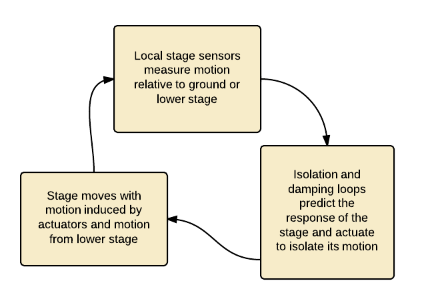
\includegraphics[scale=0.6]
	{figures/SEI_isolation_loop.png}}
	\caption{\label{fig:SEI_iso} This flowchart represents the basic feedback loop of the aLIGO active seismic isolation stages.}
\end{figure}

Advanced LIGO commissioners have demonstrated that the active seismic isolation systems so far installed perform very well in average motion during quiet seismic times - see Figure \ref{fig:HAM_ISI_current}.
However, a crucial unknown is how effectively the active seismic isolation systems mitigate transient seismic noise. Additionally, transient noise potentially introduced by the actuators themselves and how these may affect transient \gw{} searches has yet to be explored. 

\begin{figure}[htb]
\centering
\begin{subfigure}{.5\textwidth}
  \centering
  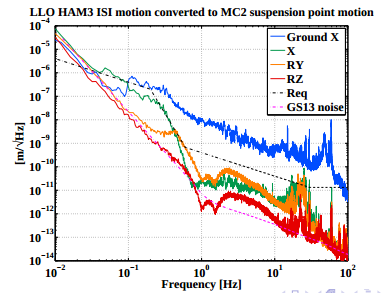
\includegraphics[width=\linewidth]{figures/Current_HAM_ISI_performance.png}
  \caption{Current HAM ISI performance spectra. Credit: R. DeRosa}
  \label{fig:HAM_ISI_current}
\end{subfigure}%
\begin{subfigure}{.5\textwidth}
  \centering
  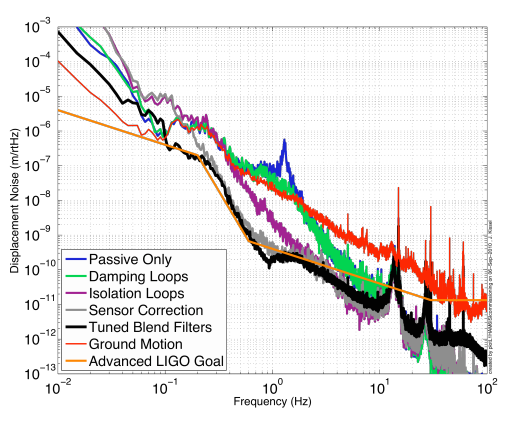
\includegraphics[width=\linewidth]{figures/SEI_SUS_spectra.png}
  \caption{aLIGO seismic noise requirements for core optics. Credit: J. Kissel.}
  \label{fig:SEISUS_spectra}
\end{subfigure}
\caption{On the left, a recent series of spectra showing the Internal Seismic Isolation (ISI) performance of an auxiliary optics chamber (known as 'HAM' or Horizontal Access Chamber'). The installed ISIs of core and auxiliary optics are currently performing better than aLIGO requirements at most frequencies in traditional average motion tests. 
On the right are spectra representing successive levels of isolation of core optic seismic isolation at design performance. Contributions from the quadruple suspensions are represented by 'Passive only'.}
\label{fig:test}
\end{figure}

\subsubsection{Suspensions}

The passive quadruple and triple suspensions provide significant seismic isolation at frequencies above 10Hz, as seen in Figure \ref{fig:SEISUS_spectra}. For active seismic isolation system characterization important to consider the active seismic isolation and suspension for each optic as complementary parts of a broader system with the same goal: to isolate the optics from local ground motion. There may sometimes be unexpected excess transient motion in the upper active isolation stages, but if this motion does not couple through the suspension masses to the motion of the optic, then it will not affect our search sensitivity. 




%%%%



\newpage
\chapter{Core-collapse supernovae}

\section{Overview}
 
\section{Leading models for CCSN explosion mechanism}


A \sn{} represents the final stage of the life cycle of a 8-130$M_\odot$ main sequence star as the fusion in the iron core burns out and the degeneracy pressure can no longer support the star against gravity. The gravitational collapse releases roughly 300 ergs of energy, 99\% in the form of neutrinos of all flavors \cite{Louge}. In 1980, Goldriech and Weber calculated a family of stable collapse configurations and showed that as the core of the star collapses, it separates into a slowly collapsing inner core and a rapidly collapsing outer core. When the inner core reaches nuclear density, it bounces into the rapidly collapsing outer core, generating a shock wave that quickly stalls from losing energy in the collision with the outer core \cite{CoreCollapse}. Neutrinos observed during the 1987 supernova have confirmed this general model \cite{SNMECH}. 

Explaining the explosion mechanism that re-energizes this shock wave and drives an explosion is the current definitive problem in \sn{} theory research. 

Three \sn{} explosion mechanisms are presently accepted in the literature as the most likely candidates: the \textit{neutrino}, \textit{magneto-rotational}, and \textit{acoustic} mechanisms \cite{Ott-SN_GWs} \todo{note that acoustic mechanism is since not believed because cannot be replicated by other groups}: 

\begin{itemize}
\item The neutrino mechanism assumes that some small fraction of the energy emitted in the form of neutrinos is absorbed in a heating effect, re-launching the stalled shock wave and producing an explosion. Recent 2D and 3D axisymmetric simulations of the neutrino mechanism have produced reliable explosions in the observed range of energies \cite{Ott-SN_GWs}, \cite{Louge}. 

\item The magneto-rotational mechanism follows from conservation of angular momentum: the collapse of the core induces a 1000x increase in rotational velocity \cite{Ott-SN_GWs} in the outer layers of the star. The differential rotation between the turbulently and rapidly rotating outer layers and slower uniform rotation of inner core could induce magnetic-field amplification that yields jet-like explosions along the axis of rotation \cite{Louge}. \footnote{Additionally, post-bounce rotational instabilities could yield asymmetric deformations of the rotating compact star, producing \gw{s} for up to hundreds of miliseconds after the initial collapse.}  

\item The acoustic mechanism begins very similarly to the neutrino mechanism, but postulates that high-velocity turbulence downflows within the post-bounce star excite quasi-periodic pulsations of the core, which develop into shockwaves that gradually (after about 1 second) build to excite an explosion. \todo{Omit all references to acoustic?}
\end{itemize}

The gravitational wave processes of the neutrino, magneto-rotational, and acoustic core-collapse supernovae explosion mechanisms are mutually exclusive, according to \cite{Ott-SN_GWs}. Thus, detecting a gravitational wave signal and classifying it by its supernovae emission process could powerfully constrain the physics of the core collapse supernovae explosion mechanism.

Examples of key waveform differences three most likely explosion mechanism models for \sn{}  can be found in Figure \ref{fig:model_waveforms}. Essentially, it is possible to confidently map the distinctive gravitational waveforms to an explosion mechanism with an accurately reconstructed and well categorized signal (see \ref{MechExtract}).

\begin{figure}[htb]
	\center{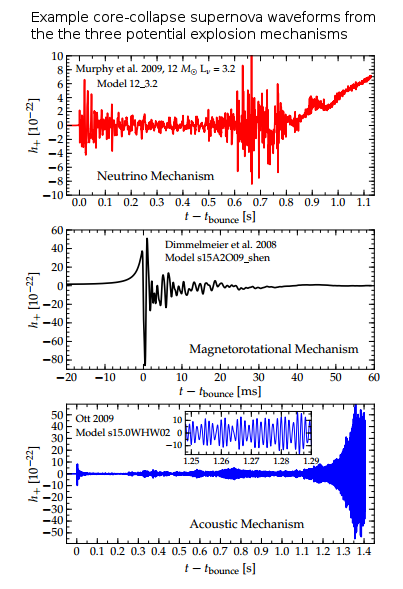
\includegraphics[scale=0.6]
	{figures/SN_waveforms.png}}
	\caption{\label{fig:model_waveforms} Examples of supernovae waveforms corresponding to the three frontrunner mechanisms for core-collapse supernovae explosion. Taken from \cite{Louge}.}
\end{figure}

%Current gravitational signal waveform catalogs for all three models are widely available. Additionally, generic waveform models for each of the three potential \sn{} mechanisms have been produced in \cite{Louge} using Principal Component Analysis and are available for comparison to \sn{} waveforms, as discussed in \ref{subsec:Classification}. 

It's also worth noting that galactic core-collapse SNe are rare events, occurring at a maximum likely rate of only a few per century. Advanced LIGO may be able to see most core-collapse SNe throughout the local group of galaxies (up to a distance of approximately 1 Mpc) \cite{Ott-SN_GWs}. 

%
%%
\section{Extracting the explosion mechanism from LIGO GW data} \label{MechExtract}

%
%%
\section{The importance of waveform reconstruction} 

\newpage
\chapter{Detecting and reconstructing CCSN signals from aLIGO data }

\section{The burst all-sky search and transient detection} 
\section{Overview of reconstruction methods} 
\subsection{cWB2G} 
\subsection{BayesWave}
\subsection{(MaxEnt??)} 

%
%%
\section{Comparison of reconstruction methods}
\subsection{Technique }
\subsection{Results }

\newpage
\chapter{Characterizing and mitigating terrestrial noise sources} \label{c:DetChar}

\section{Characterizing general transient noise } 

Event trigger generators, or ETGs, are essential tools for evaluating transient noise in auxiliary channels, including seismic channels. ETGs identify periods of excess signal, often referred to as \textit{glitches}, and calculate useful characteristics about these features like central time, central frequency, and amplitude.

\subsection{Performance of single interferometer burst pipelines}
The ETG Omicron, which I have chosen to use for seismic transients studies for reasons shown in Figure \ref{fig:ETGs}, works by the following procedure: 
\begin{enumerate}
\item Data is projected onto a sine-gaussian basis via tiling in time, frequency, and Q (number of cycles of the signal).
\item Data is whitened by the median-mean power spectral density (robust to transient noise pollution) 
for some time segment known as \textit{block duration}.
\item The most significant tile becomes an Omicron trigger with 
associated time, frequency, Q, and amplitude. 
\end{enumerate}

As an example of the studies performed so far, I compared the detection efficiency of different ETGs for a range of plausible \gw{} waveforms (sine gaussians, ring downs, and core-collapse supernovae waveforms generated with numerical simulations). Figure~\ref{fig:ETGs} shows that Omicron and Omega detect nearly 100\% of all injected signals, as expected. The study also showed that for detected signals, Omicron and Omega also outperform ExcessPower in reconstructing trigger parameters like central time and SNR. 
 
\begin{figure}[htb]
	\center{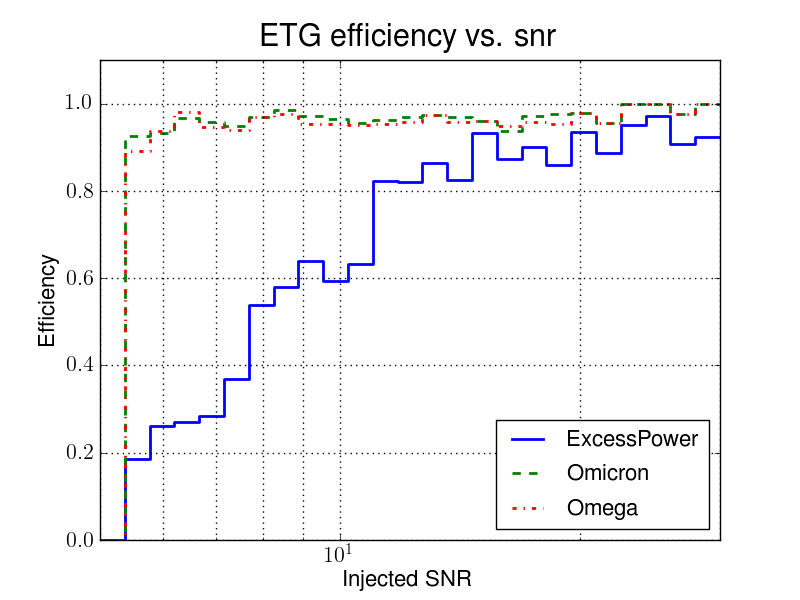
\includegraphics[scale=0.4]
	{figures/ER3_efficiency_vs_snr.png}}
	\caption{\label{fig:ETGs} Efficiency vs. SNR for the three algorithms that are being considered by the collaboration as potential single interferometer burst search pipelines (Omicron, Omega, and ExcessPower)}.
\end{figure}


We still need to optimize Omicron's running parameters for the identification of seismic noise transients at low frequency (0.1-10Hz), as previous ETG studies targeted the aLIGO search band (see Figure \ref{fig:ETGs}). 
A remaining hurdle, as shown in \cite{Macleod-Seisveto} is that ETGs require significant tuning away from their standard parameters in order to resolve the low frequency, long duration transients commonly seen in seismic sensors - see Figure \ref{fig:OmicronTuning} for an example of this. 
In terms of Omicron parameters, this will likely require using much longer block duration than the standard configuration of 32s for whitening, as we want enough data to resolve features that could potentially have durations of tens or hundreds of seconds. \todo{DONE?}


%
%%
%%%
\section{Seismic noise}

\subsection{Livingston train up-conversion} 


Seismic noise from the nearby train at Livingston was a common problem for transient \gw{} searches during the previous science run. 
We discovered that the 1-3Hz seismic noise produced by the train does couple into the PRMI Power Recycling Cavity Length signal (see Figure \ref{fig:aLIGOconfig}) at frequencies within the \gw{} search band (20-40Hz) - see Figure \ref{fig:TRAIN}). 
\todo{Replace all with DARM results!!}

\begin{figure}[htb]
\centering
\begin{subfigure}{.48\textwidth}
  \centering
  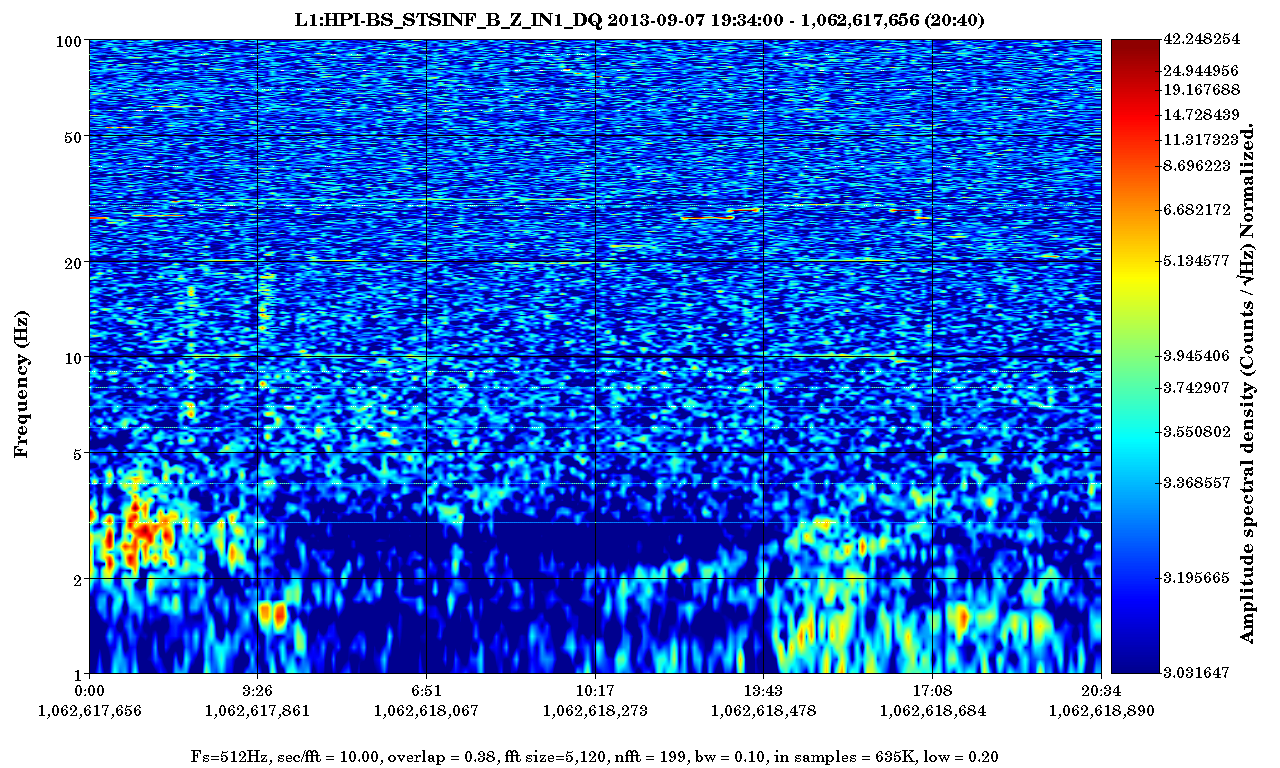
\includegraphics[width=\linewidth]{figures/GroundMotionSpec.png}
  \caption{Ground motion}
  \label{fig:TrainGroundSpec}
\end{subfigure}%
\begin{subfigure}{.48\textwidth}
  \centering
  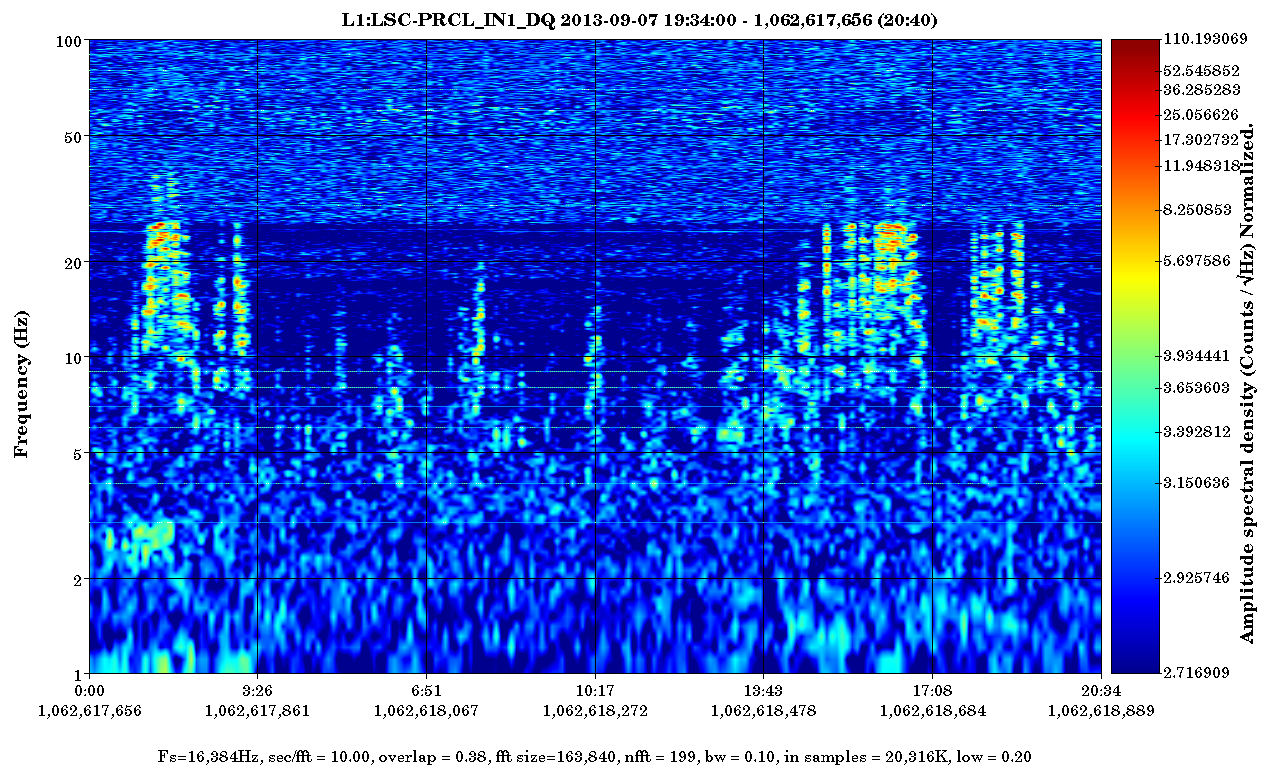
\includegraphics[width=\linewidth]{figures/PRMI_PRCL_spec.png}
  \caption{PRMI control signal}
  \label{fig:TrainPRCL}
\end{subfigure}
\caption{Normalized spectrograms of a recent 20 minute Livingston PRMI lock time during which a train was passing through within the first three minutes. Ground motion is on the left, and the Power Recycled Cavity Length signal (control signal for the PRMI) is on the right. The frequency scale is the same for both plots. Note that the quieter ground motion from minutes 13-20 (roughly half the amplitude of the train motion) also produces significant upconverted noise in the PRMI signal.}
\label{fig:TRAIN}
\end{figure}

\section{Advanced LIGO seismic noise transient propagation}

SEI transient study results 

\begin{figure}[htb]
\centering
\begin{subfigure}{.45\textwidth}
  \centering
  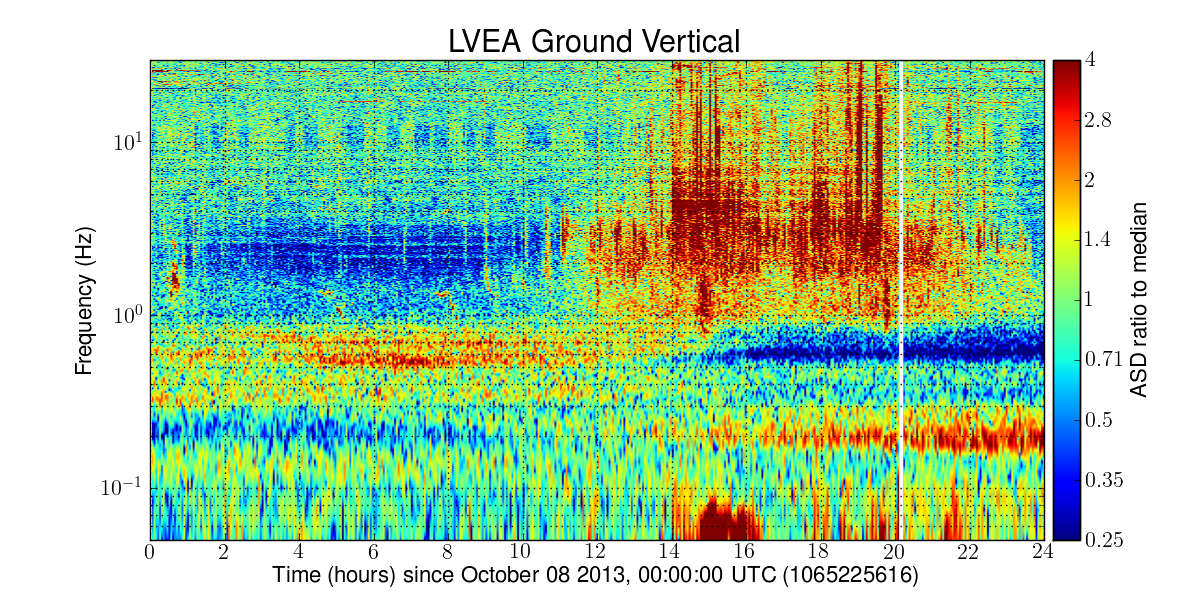
\includegraphics[width=\linewidth]{figures/Spectro_ground.png}
  \caption{Recent normalized spectrogram of Z-direction of ground motion sensors at Livingston}
  \label{fig:groundZspec}
\end{subfigure}%
\begin{subfigure}{.45\textwidth}
  \centering
  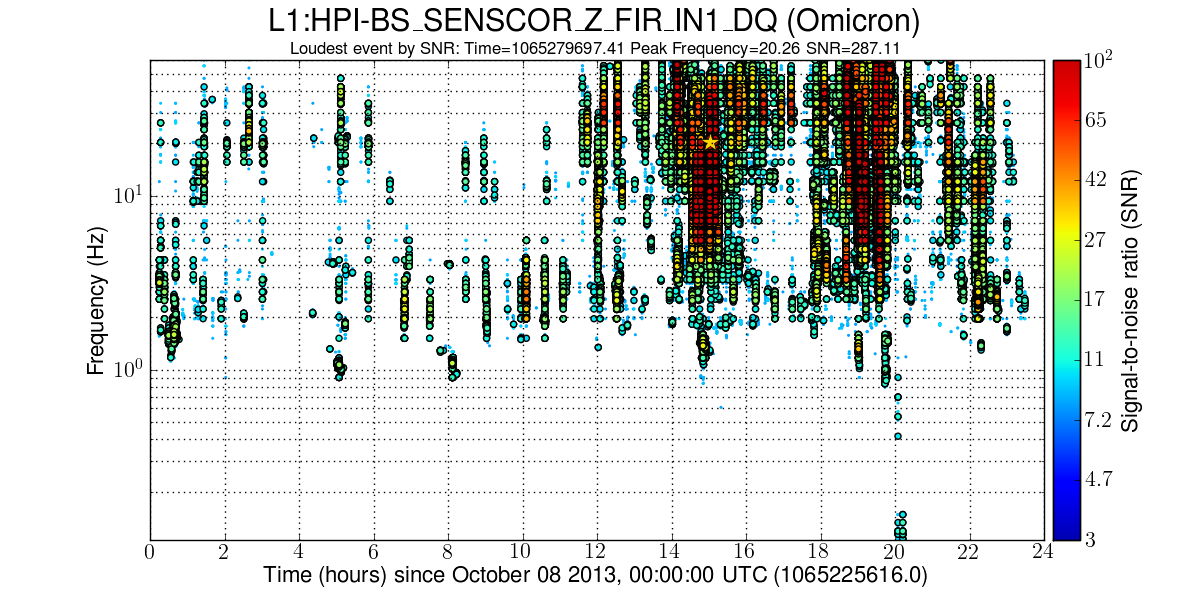
\includegraphics[width=\linewidth]{figures/Omicron_ground.png}
  \caption{Omicron triggers for the same channel during the same time period, before parameter tuning.}
  \label{fig:groundOmicron}
\end{subfigure}
\caption{A comparison of a recent normalized spectrogram of a Livingston ground motion sensor and Omicron triggers for the corresponding time - before parameter tuning. Note the low frequency structure seen below 1Hz in the normalized spectrogram is not seen by Omicron.}
\label{fig:OmicronTuning}
\end{figure}

Once Omicron is fully configured to resolve seismic transients, resolving transient noise in seismic sensor channels with good accuracy will be possible. I intend to use this tool in critical seismic transient studies (see~\S\ref{s:proposed}). 

All of these sensors have different units and ranges of validity. Tools used to analyze these channels for transient noise, or Event Trigger Generators, need to be tuned for each set of sensors in order to produce accurate trigger parameters like central time, frequency, and amplitude for transient events in these channels. 

\section{Techniques for transient noise mitigation}

%
%%
\subsection{Data quality vetoes}

\begin{figure}[htb]
	\center{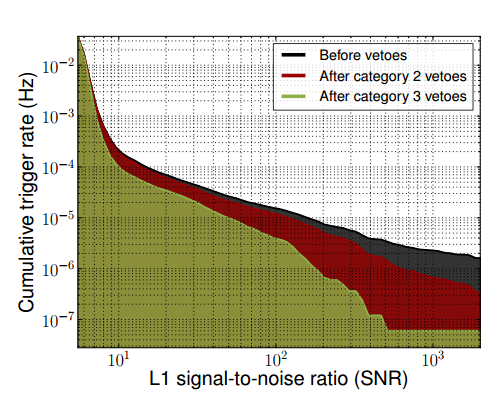
\includegraphics[scale=0.4]
	{figures/S6DQVetos.png}}
	\caption{\label{fig:S6DQ} An excerpt figure from the upcoming S6 detector characterization paper that draws heavily on the work I performed evaluating the performance of data quality flags, which are lists of time segments corresponding to pre-defined states of the detector. Data quality flags that indicate states where detection isn't possible are grouped together into 'categories' where lower category numbers indicate a more severe known problem. Categories 1 and 2 were removed from all transient \gw{} searches. Note the non-Gaussanity of this S6 Livingston distribution of single-detector burst search triggers after the removal of categories 1, 2 and 3.\todo{Check this is still current version of this figure with new detchar paper.}}
\end{figure}

%
%%
\subsection{Event-based veto generation}  

hveto, 




%%%%%%
%\subsection{Coherence studies} 
%
%A common follow-up to investigate potential couplings when the source of the noise is unknown is a coherence matrix, as shown in Figure \ref{fig:coherence}. For each matrix, the coherence between a list of interesting auxiliary channels indicative of potential noise couplings and the control signal (or channel of interest) is calculated for each 0.1 Hz frequency bin and plotted in a matrix form to easily spot potential correlations. Many configurations of this coherence matrix exist to target different subsystems, and I have developed those for the seismic isolation and suspensions systems. 
%
%As an example, the detector characterization group was recently requested by the Livingston site commissioners to investigate the source of unexpected excess noise below 1Hz in the PRMI signal.
%Our results (in Figure \ref{fig:coherence}) showed coherence of the ISI (Internal Seismic Isolation platforms) motion in HAM (auxiliary optics) chambers 2 and 3 and the suspension motion of optics in the same chamber with the PRMI control signal. The commissioners were able to use these results to isolate the problem and tune the ISI active seismic isolation loops to remove the excess noise. 
%
%\begin{figure}[htb]
%	\center{\includegraphics[scale=0.45]
%	{figures/CoherenceMatrix.png}}
%	\caption{\label{fig:coherence} Coherence of selected active seismic isolation platform motion sensors and suspension motion sensors with the PRMI control signal (PRCL) calculated for each 0.1 Hz wide frequency bin. Coherence with the PRMI signal was found for ISI (Internal Seismic Isolation platforms) motion and suspension motion in HAM (auxiliary optics) chambers 2 and 3 in the frequency range of the unknown noise source. } 
%\end{figure}

% --------------------------------------------------------------------------------------

%% -----------------------------------------------------------------------------------------
%% -----------------------------------------------------------------------------------------
%% -----------------------------------------------------------------------------------------
%% -----------------------------------------------------------------------------------------



\newpage
\chapter{The impact of terrestrial seismic noise on CCSN detectability and reconstruction}

\section{CCSN detectability in recolored non-Gaussian data}
Simple cWB runs on CCSN waveforms scaled to different distances (detection efficiency versus distance) 
\section{CCSN reconstruction in recolored non-Gaussian data}
Waveform reconstruction results for ONE method in Gaussian data versus S5 data recolored to aLIGO expected strain

\newpage
\chapter{Conclusions and future prospects}

High rates of transient noise will have a significant impact of CCSN detectability and waveform reconstruction - must be a top priority to mitigate it 
% -------------------------------------------------------------------------------- 







%% End of body
%%%%%%%%%%%%%%%%%%%%%%%%%%%%%%%%%%%%%%%%%%%%%%%%%%%%%%%%%%%%%%%%%%%%%%%%%%%%%%%

%\appendix


%\chapter{THE SECOND APPENDIX TITLE}
%...

%%
%% Beginning of back matter
\backmatter  %% <--- mandatory

%%
%% We don't support endnotes

%%
%% A bibliography is required.
\interlinepenalty=10000  % prevent split bibliography entries
\bibliographystyle{umthesis}
\bibliography{umthsmpl}
\end{document}

%%% Local Variables: 
%%% mode: latex
%%% TeX-master: t
%%% End: 
